\chapter{Configuring VNC Access}

\section{Understanding VNC}
Virtual Network Computing (VNC) is a graphical desktop sharing system that lets a remote user control a local server. On our server runs a Graphical User Interface (GUI) provided by \textbf{X-Server} (which handles all graphical I/O and graphics processing interfaces). While the X-Server is capable of providing a single GUI to the local user, it's also the system service responsible for providing VNC interfaces. 

VNC doesn't take over the existing GUI session. Instead, it provides a second GUI session for the remote user, which also runs on top of X-Server. For this to be possible, there must be a VNC server process running on our server. 

Let us consider a remote user connects for a VNC session using VNC viewer via \verb|user@host localhost:1|, through SSH (and is thus received by \verb|sshd|). The SSH protocol is needed as VNC itself is insecure. Sending clear-text id and passwords over the network is extremely ill-advised, and thus the user should initiate an encrypted session with the ssh process. Once the user has authenticated with SSH, a session can be established from SSH to the VNC server. 

\begin{figure}[H]
	\centering
	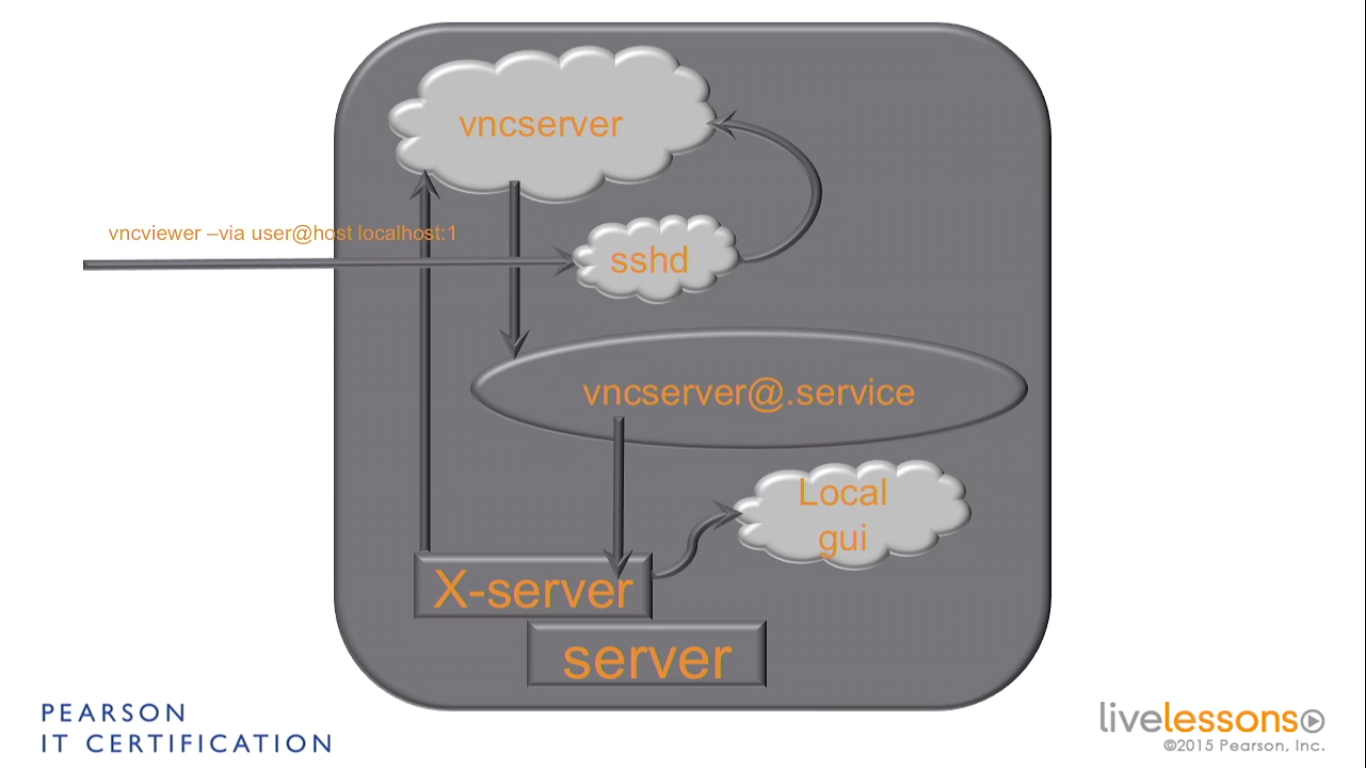
\includegraphics[width=0.9\linewidth]{RHCSA/Mod4/chapters/4.26.a}
	\caption{VNC Connection}
	\label{fig:4 VNC Connection}
\end{figure}


Next, a connection will be established from the VNC server to the VNC session running for that user. This session will provide access to the X-Server, thus making it possible for the remote user to with a full-blown graphical user interface running on the server. 

\section{Configuring a VNC Server}
The main difficulty in setting up a functional VNC server comes from the fact that there are a lot of tiny components that need to work together to make the session work. First we need to install \textbf{tigervnc} and \textbf{tigervnc-server}. TigerVNC is the client and the other package, the VNC server. 

To use VNC, we need to specify the settings for a particular user. For this we add a user called \textit{vncuser}, and add a password for it, since it's  going to connect through an SSH session. 

\vspace{-15pt}
\begin{minted}{console}
# useradd vncuser
[root@vmPrime ~]# passwd vncuser
Changing password for user vncuser.
New password: 
BAD PASSWORD: The password fails the dictionary check - it is based on a dictionary word
Retype new password: 
passwd: all authentication tokens updated successfully.
\end{minted}
\vspace{-10pt}

\subsection{Creating the VNC Server Configuration File}
In the \verb|/usr/lib/systemd/system| directory, there is a file named \verb|vncserver@.service|. We need to copy and rename it to:

\vspace{-15pt}
\begin{minted}{console}
# cp vncserver@.service vncserver@\:1.service
# ls vncserver*
vncserver@:1.service  vncserver@.service
\end{minted}
\vspace{-10pt}

\noindent
The \verb|\| in the name of the file is just used as an escape character to provide the \verb|:| in the file name \verb|vncserver@:1.service|. The number $1$ in the file name is the number of the VNC session ($1^{st}$) that we want to provide. The session number must start from 1 onwards, since the service will refuse to start for session number 0. Now, we modify the contents of the file we just created. There are sections in the file that contain placeholders called \verb|<USER>| which must be replaced with the actual username that we just created:

\vspace{-15pt}
\begin{minted}{bash}
[Unit]
Description=Remote desktop service (VNC)
After=syslog.target network.target

[Service]
Type=forking
User=vncuser	# There was a placeholder <USER> here

# Clean any existing files in /tmp/.X11-unix environment
ExecStartPre=-/usr/bin/vncserver -kill %i
ExecStart=/usr/bin/vncserver %i
PIDFile=/home/vncuser/.vnc/%H%i.pid	# There was a placeholder <USER> here
ExecStop=-/usr/bin/vncserver -kill %i

[Install]
WantedBy=multi-user.target
\end{minted}
\vspace{-10pt}

\noindent
Now, systemd needs to be notified that a new configuration file has been added. We use the \verb|systemctl daemon-reload| which causes systemd to reload all unit files, in which our new service will also be loaded. 

\vspace{-15pt}
\begin{minted}{console}
# systemctl daemon-reload
\end{minted}
\vspace{-10pt}

\noindent
Finally, before starting the VNC server session, we must set a VNC password for \textit{vncuser}. Note that this can only be done as the VNC user, and \textbf{NOT} as root, even though RedHat documentation may suggest it. 

\vspace{-15pt}
\begin{minted}{console}
# su - vncuser
$ vncpasswd
Password:
Verify:
Would you like to enter a view-only password (y/n)? n
$ exit
logout
\end{minted}
\vspace{-10pt}

\noindent
Now, the VNC environment has been setup for \textit{vncuser}, and we can start the VNC server.

\vspace{-15pt}
\begin{minted}{console}
# systemctl start vncserver@\:1
# systemctl status vncserver@\:1
● vncserver@:1.service - Remote desktop service (VNC)
Loaded: loaded (/usr/lib/systemd/system/vncserver@:1.service; disabled; vendor preset: disabled)
Active: active (running) since Fri 2017-12-22 21:38:20 IST; 26s ago
Process: 17085 ExecStart=/usr/bin/vncserver %i (code=exited, status=0/SUCCESS)
Process: 17076 ExecStartPre=/usr/bin/vncserver -kill %i (code=exited, status=2)
Main PID: 17101 (Xvnc)
CGroup: /system.slice/system-vncserver.slice/vncserver@:1.service
├─17101 /usr/bin/Xvnc :1 -auth /home/vncuser/.Xauthority -desktop vmPrime.somuVMnet.com:1 (vncuser) -fp catalogue:/etc/X11/fontpath.d -geometry 1024x768 -pn -rfbauth /home/vncuser...
├─17106 /usr/libexec/gnome-session-binary --session=gnome-classic
...
\end{minted}
\vspace{-10pt}

\noindent
Now we need to allow the service through the firewall. Firewalls in generals are more permissive for outgoing connections than incoming connections. 

\vspace{-15pt}
\begin{minted}{console}
# firewall-cmd --permanent --add-service=vnc-server
success
# firewall-cmd --reload
\end{minted}
\vspace{-10pt}

\noindent
The last command, \verb|firewall-cmd --reload| causes firewalld to reload it's configuration. This is all the setup needed on the VNC server. 

Thus the steps to setup a VNC server can be boiled down to:

\begin{figure}[H]
	\centering
	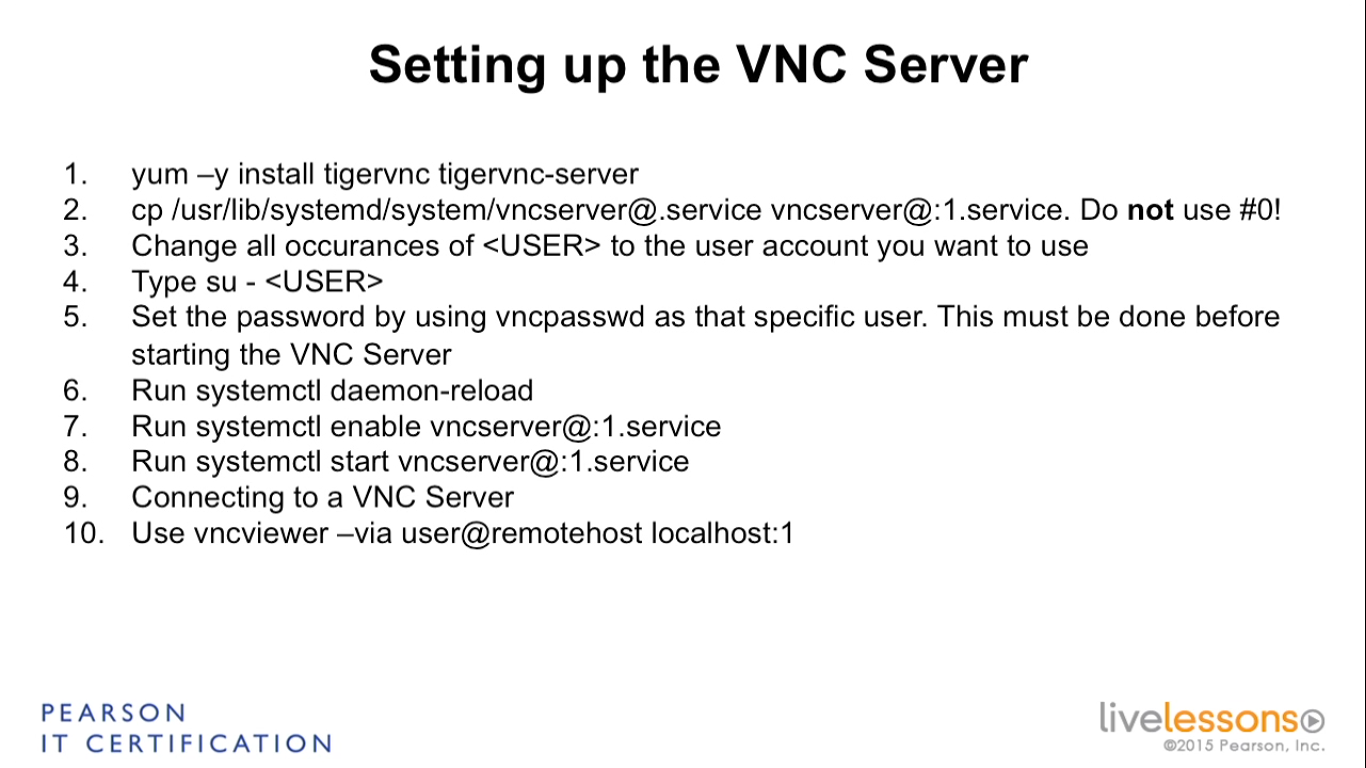
\includegraphics[width=0.9\linewidth]{RHCSA/Mod4/chapters/4.26.b}
	\caption{Steps for VNC Server config}
	\label{fig:4 Steps for VNC Server config}
\end{figure}

\section{Connecting to a VNC Server}
To connect to the VNC server, we need the \textbf{vncviewer} utility. The basic syntax of the \verb|vncviewer| command is: \verb|vncviewer -via <vnc-username>@<vnc-host> <vnc-host>:1|. So, when testing it on localhost, we'll use:

\vspace{-15pt}
\begin{minted}{console}
# vncviewer -via vncuser@localhost localhost:1

TigerVNC Viewer 64-bit v1.8.0
Built on: 2017-12-01 23:20
Copyright (C) 1999-2017 TigerVNC Team and many others (see README.txt)
See http://www.tigervnc.org for information on TigerVNC.
vncuser@localhost's password: 

Sat Dec 23 19:13:38 2017
DecodeManager: Detected 1 CPU core(s)
DecodeManager: Decoding data on main thread
CConn:       connected to host localhost port 33955
t CConnection: Server supports RFB protocol version 3.8
CConnection: Using RFB protocol version 3.8
CConnection: Choosing security type VeNCrypt(19)
CVeNCrypt:   Choosing security type TLSVnc (258)
e
Sat Dec 23 19:13:41 2017
CConn:       Using pixel format depth 24 (32bpp) little-endian rgb888
CConn:       Using Tight encoding
CConn:       Enabling continuous updates
\end{minted}
\vspace{-10pt}

\noindent
When the above command is executed, first SSH authentication occurs, followed by VNC authentication. If both authentications are passed, a remote session on the server for that particular user (i.e., \textit{vncuser} in our case) is started. 